%% SECTION HEADER /////////////////////////////////////////////////////////////////////////////////////
\section{Determination of the MADIF}
\label{sec:determination}

%% SECTION CONTENT ////////////////////////////////////////////////////////////////////////////////////
The \ac{madif} is determined based on the numerical index best fitted to the experimental one. 
For that reason, the error between the numerical and experimental obtained indices was determined in the form of:
\begin{eqnarray}
	error = \sum_{i=1}^{\mathrm{n^{DI}}} \left|\frac{\mathrm{DI_i^{num}}-\mathrm{DI_i^{exp}}}{\mathrm{DI_i^{exp}}}\right|\times\frac{100}{\mathrm{n^{DI}}}\%,
\end{eqnarray}
where \(\mathrm{n^{DI}}\) is number of the index points.
The error values are shown in Fig. \ref{fig:bar_f} for all the \acp{di} based on the full core model and Fig. \ref{fig:bar_h} for all the \acp{di} based on the homogenised core model.
The \ac{rmsd} occurred best index for both models, at 50 kHz for the simplified core and 100 kHz for the full core model.
\begin{figure}[!tbh]
	\begin{center}
		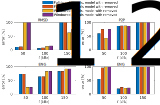
\includegraphics{Chapter_7/bar_f}
	\end{center}
	\caption{Percentage error of the \acp{di} for the full core model.}
	\label{fig:bar_f}
\end{figure}
\begin{figure}[!tbh]
	\begin{center}
		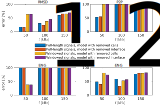
\includegraphics{Chapter_7/bar_h}
	\end{center}
	\caption{Percentage error of the \acp{di} for the homogenised core model.}
	\label{fig:bar_h}
\end{figure}
The indices are used to determine the \ac{madif} for the analysed panel, assuming it is a non-linear approximation function in the form:
\begin{eqnarray}
	\mathrm{MADIF(DI)} = \frac{a_1\mathrm{DI}}{\mathrm{DI}-a_2},
	\label{eg:app_function} 
\end{eqnarray}
where \(a_1\) and \(a_2\) are the coefficients of the function fitted to the values obtain in the numerical simulations. The coefficients are determined by built-in function of Matlab named \verb+fminsearch+, which searches for the minimum of a problem specified by \(\min\limits_x f(x)\).
In the case of this model, the number of \ac{rmsd} points was limited to \(\mathrm{n^{DI}}=4\) as the index reached its maximum value and decreased above the fourth damage size.
Fit curves for \(\mathrm{n^{DI}}=4\) to \(\mathrm{n^{DI}}=7\) are presented in Fig. \ref{fig:RMSD_F}. 
For the homogenised core model, the \ac{madif} is obtained for seven points as the \ac{rmsd} increases monotonically in the full range of damage.
Fit curve for \(\mathrm{n^{DI}}=7\) is presented in Fig. \ref{fig:RMSD_H}.
\begin{figure}[!tbh]
	\begin{center}
		\includegraphics{Chapter_7/RMSD_100kHz_F}
	\end{center}
	\caption{RMSD}
	\label{fig:RMSD_F}
\end{figure}
\begin{figure}[!tbh]
	\begin{center}
		\includegraphics{Chapter_7/RMSD_50kHz_H}
	\end{center}
	\caption{RMSD}
	\label{fig:RMSD_H}
\end{figure}
\begin{figure}[!tbh]
	\begin{center}
		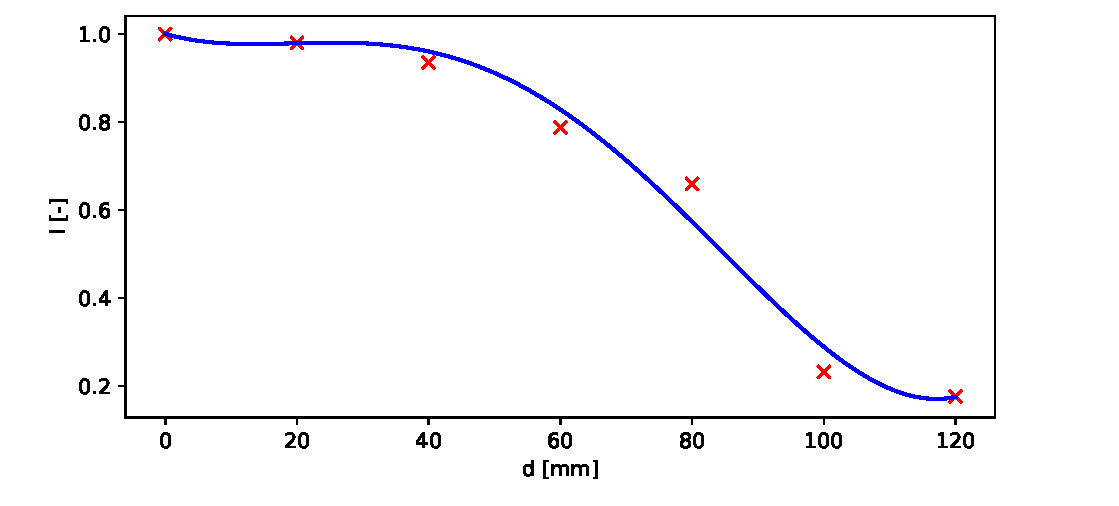
\includegraphics{Chapter_7/madif}
	\end{center}
	\caption{\ac{madif}}
	\label{fig:madif}
\end{figure}

Based on the results obtained, the determined \ac{madif} takes values for the full model:
\begin{eqnarray}
	\mathrm{w_d} = \mathrm{MADIF(DI)} = \frac{15.19\mathrm{DI}}{\mathrm{DI}-0.87},
	\label{eg:madif_full} 
\end{eqnarray}
and for the homogenised model:
\begin{eqnarray}
	\mathrm{w_d} = \mathrm{MADIF(DI)} = \frac{16.33\mathrm{DI}}{\mathrm{DI}-1.42}.
	\label{eg:madif_homog} 
\end{eqnarray}
Both functions are shown in Fig. \ref{fig:madif}, along with the given absolute error as the difference in the \ac{madif} value from the measured one \(\Delta \mathrm{w_d}=\left|w_d^{MADIF}-w_d^{experimental}\right|\) [mm].
It can be noticed that approximation functions are in good agreement with experimental results.
In the case of the full core model case, all errors are \(\Delta \mathrm{w_d}\leq26\) [mm], except for the last argument the function has an unsatisfactory value with \(\Delta \mathrm{w_d}=55\) [mm].
Such a significant error may be since the function for large defects is abrupt and asymptotically tends maximal damage size \(\mathrm{w_d}=200\) [mm]. 
Therefore, even small changes in the index in this range will cause a considerable change in the defect value.
In the case of the homogenised model, last two values are out of the scale the errors are lest than \(\Delta \mathrm{w_d}\leq24\) [mm].
In the case of the homogenised model, the last two values are out of the scale, as the experimental measurements are higher than an asymptote of the \ac{madif}, defined by \ac{rmsd}=1.41.
The errors for the all points before the asymtote are \(\Delta \mathrm{w_d}\leq24\) [mm].
